

\begin{enumerate}
    \begin{minipage}[t]{0.35\linewidth}
        \textbf{M1204*}. На плоскости заданы точки A, B, C --- центры трех кругов. Каждый круг равномерно раздувается (радиус увеличивается с одинаковой для всех кругов скоростью). Как только два круга касаются друг друга, они "лопаются" --- их радиусы уменьшаются до 0 --- и начинают расти снова. Верно ли, что если расстояния AB, BC, CA --- целые числа, то этот процесс будет периодическим?

        Изучите, как может развиваться этот процесс, если треугольник ABC а) равносторонний; б) равнобедренный; в)* прямоугольный со сторонами 3, 4, 5.

        Начальное состояние может быть произвольным (не только "нулевым").

        \begin{minipage}[c]{\textwidth}
        \centering
            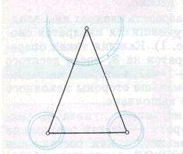
\includegraphics[width=\linewidth]{pic1.png}
            \caption{Рис. 1.}
            \label{fig:pic1}
        \end{minipage}

        \begin{minipage}[c]{\textwidth}
        \centering
            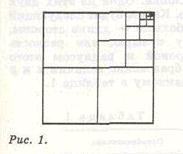
\includegraphics[width=\linewidth]{pic2.png}
            \caption{Рис. 2.}
            \label{fig:pic2}
        \end{minipage}
    \end{minipage}

    \hspace{0.05\textwidth}

    \begin{minipage}[t]{0.6\linewidth}
        Будем рассматривать общий случай: исходные радиусы пузырей произвольны.
        а) Треугольник ABC равносторонний. После первого хлопка радиусы двух пузырей будет равны нулю. При втором хлопке лопнут все три пузыря. Затем процесс будет периодически повторяться.

        б-1) Треугольник ABC равнобедренный, основание меньше боковой стороны. Тогда при первом или втором хлопке лопнут два пузыря, центры которых лежат в основании треугольника. Далее их радиусы будут равны (рис. 1). Вскоре лопнут одновременно все три пузыря, после чего начинается периодический процесс. Количество хлопков в периоде (цикле) зависит от отношения длин боковой стороны и основания.

        Теперь рассмотрим с более общих позиций оставшиеся случаи: б-2) (основание больше боковой стороны) и в). Мы увидим, что в этих случаях процесс, как правило, не будет периодическим.

        Обозначим длины отрезков BC, AC и AB через a, b и c соответственно. Пусть для определенности $a \leqslant b < c$. (Вариант $b=c$ мы уже рассмотрели.) Заметим, что пузыри с центрами в точках A и B (короче: пузыри A и B) могут соприкоснуться разве лишь в самом начале процесса. После этого в каждом хлопке участвует пузырь C. Таким образом, конкретное значение величины c не играет никакой роли (лишь бы выполнялось условие $b<c$). Понятно также, что важны не сами по себе длины a и b, а их отношение $r=b/a$. Поэтому будем в дальнейшем рассматривать треугольник ABC с боковыми сторонами BC=1, AC=$r \geq 1$ и основанием AB>r.

        Обозначим через x и y радиусы пузырей A и B сразу после произвольного хлопка. Одна из этих двух величин заведомо равна нулю. Каким будет следующий хлопок, зависит от того, что больше --- длина стороны, противолежащей уцелевшему пузырю, или разность между другой боковой стороной и радиусом этого пузыря. Таким образом, преобразование величин x и y происходят по правилу, указанному в \ref{table:table1}.

        \bgroup
        \def\arraystretch{1.5}

        \begin{center}
            \captionof{table}{Преобразования}
            \label{table:table1}
            \begin{tabular}{ c | c | c }
                \hline
                 & Текущее состояние & Преобразование \\
                \hline
                1 & $y=0, r-x>1$ & $x_\textup{нов}=x+\frac{1}{2}, y_\textup{нов}=0$ \\ 
                \hline
                2 & $y=0, r-x=1$ & $y_\textup{нов}=0, x_\textup{нов}=0$ \\
                \hline
                3 & $y=0, r-x<1$ & $y_\textup{нов}=(r-x)/2, x_\textup{нов}=0$ \\
                \hline
                4 & $x=0, 1-y<r, y \neq 0$ & $x_\textup{нов}=(1-y)/2, y_\textup{нов}=0$ \\
                \hline
            \end{tabular}
        \end{center}

        \egroup
    \end{minipage}
\end{enumerate}
